Since the Einstein Telescope is currently still in its planning stages, no real detector data exist, with which neural networks can be trained and tested. 
Thus, a considerable amount of this thesis' work has been spent on simulating gravitational wave signals, and the corresponding detector response under realistic noise conditions. 
In the context of machine learning, such simulated data is commonly referred to as \emph{synthetic} data.

This chapter provides a detailed description of the simulation of detector noise and GW signals, as well as the construction of samples to form datasets.
Most of the utilities required for these simulations are provided by the PyCBC software package \cite{alex_nitz_2023_10013996}, and the hardware was provided by the PALMA II HPC of the University of Münster.

\section{Detector Noise}
\label{sec:data_simulation:noise}
\begin{figure}
	\centering
	\makebox[\textwidth]{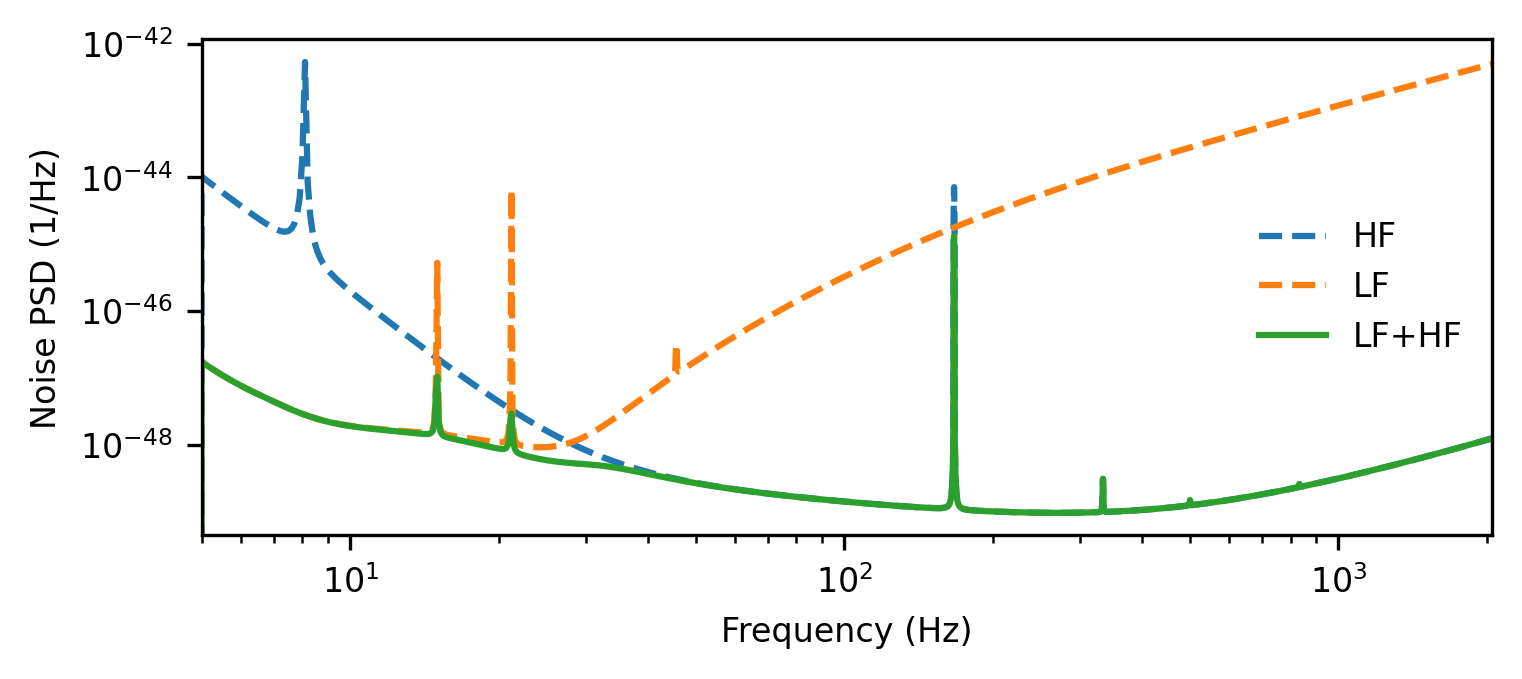
\includegraphics[width=13cm]{data_simulation/images/ET-0304B-22/18213_ET10km.png}}
	\caption{The ET noise PSD of the LF and HF interferometers, and of their combination (LF+HF), which is the PSD employed in this work. The PSDs are plotted from \SI{4}{\hertz} to \SI{2048}{\hertz}, corresponding to the simulation upper and lower frequency range. Data taken from \cite{ET-0304B-22}.}
	\label{fig:data_simulation:noise_psd}
\end{figure}

This thesis assumes the detector noise to be \emph{Gaussian}, meaning it has amplitudes, which are normally distributed. The noise is then fully characterized by the noise power spectral density (PSD). See Ch.~\ref{sec:matched_filtering} for further information. This thesis employs the sensitivity of ET according to the latest design report \cite{ET-0007C-20} in a triangular configuration with \SI{10}{\kilo\meter}-long arms (see Ch.~\ref{sec:einstein_telescope}).
The corresponding PSD data are taken from \cite{ET-0304B-22}, which provides the noise PSDs for the LF and HF interferometers in the frequency range from \SI{1}{\hertz} to \SI{10}{\kilo\hertz}, as well as for their
combined sensitivity (LF+HF).
The combined PSD is obtained through, 
\begin{equation}
	\frac{1}{S_n^\text{LF+HF}(f)} = \frac{1}{S_n^\text{LF}(f)} + \frac{1}{S_n^\text{HF}(f)}.
\end{equation} 
The corresponding PSD curves are shown in Fig.~\ref{fig:data_simulation:noise_psd}.
In this work, the intricacies of the xylophone configuration, where each detector consists of two nested interferometers, are ignored. Instead, ET is treated as three interferometers in a triangular configuration, assuming the ET LF+HF noise PSD for each. 

Such noise is called \emph{colored}, because its power spectrum is \emph{not} constant over the whole frequency regime (in contrast to \emph{white} noise with a flat power spectrum), and \emph{stationary} because the power spectrum stays constant with respect to time. Notice that for currently operating GW interferometers such as LIGO and Virgo their noise is typically non-stationary. This is due to slow drifts in the PSD over minutes or hours and because of short-duration transient noise events called \emph{glitches} \cite{Abbott_2020}. Regardless, in this work the detectors' noise is assumed to be stationary, since it is not entirely clear if and how exactly non-stationarity might arise.

In the proposed ET xylophone configuration, some of the interferometers' test masses will be located less than a few \SI{100}{\meter} apart, which is why a non-negligible correlation is expected among the noise of the detectors in the form of seismic noise, especially in the low-frequency regime up to \SI{\sim40}{\hertz} \cite{PhysRevD.109.102002}. Currently, there is no routine implemented in PyCBC for the simulation of correlated noise. Instead, this is done from scratch following the approach in \cite{PhysRevD.110.104060}. The algorithm will be presented by first describing how uncorrelated noise is simulated from a given power spectrum, and then showing how this procedure is adapted in the case of correlated noise.

\subsection*{Uncorrelated Noise}

Consider a noise time-series $n = (n(t_0), n(t_1), \dots)$ that is to be simulated for one detector with a PSD $S_n = (S_n(f_0), S_n(f_1), \dots)$. The discrete Fourier transform of that time-series $\tilde{n} = (\tilde{n}(f_0), \tilde{n}(f_1), \dots)$ should then satisfy,
\begin{equation}
	\label{eq:data_simulation:psd_relationship}
	\frac{1}{2}S_n(f) = \Delta f\bigl\langle|\tilde{n}(f)|^2\bigr\rangle, 
\end{equation}
where $\Delta f$ is the frequency resolution. This follows from the PSD definition (Eq.~\ref{eq:matched_filtering:PSD_definition}), as evaluated over a constant observation time $T$, in discrete form. Requiring the noise to be Gaussian, motivates an ansatz of the form,
\begin{equation}
	\label{eq:data_simulation:uncorrelated_noise_dft_ansatz}
	\tilde{n}(f) = a (x + iy), 
\end{equation}
where $x$ and $y$ are drawn from a normal distribution with zero mean and unit variance, $x, y \sim \pazocal{N}(\mu=0, \sigma^2=1)$, and where $a$ is some arbitrary prefactor. Since the expectation value of a squared normal random variate is one, $\bigl\langle|\tilde{n}(f)|^2\bigr\rangle = a^2 (\langle x^2\rangle + \langle y^2\rangle)$ simplifies to $2 a^2$, and thus with Eq.~\ref{eq:data_simulation:psd_relationship},
\begin{equation}
	\label{eq:data_simulation:prefactor}
	a = \frac{1}{2}\sqrt{\frac{S_n(f)}{\Delta\!f}}.
\end{equation}
That is, the discrete Fourier transform of the noise has a uniformly random phase and a magnitude, which is, on average, proportional to the square root of the noise PSD. Finally, $n$ can be computed as the inverse discrete Fourier transform of $\tilde{n}$.

\subsection*{Correlated Noise}

\begin{figure}
	\centering
	\makebox[\textwidth]{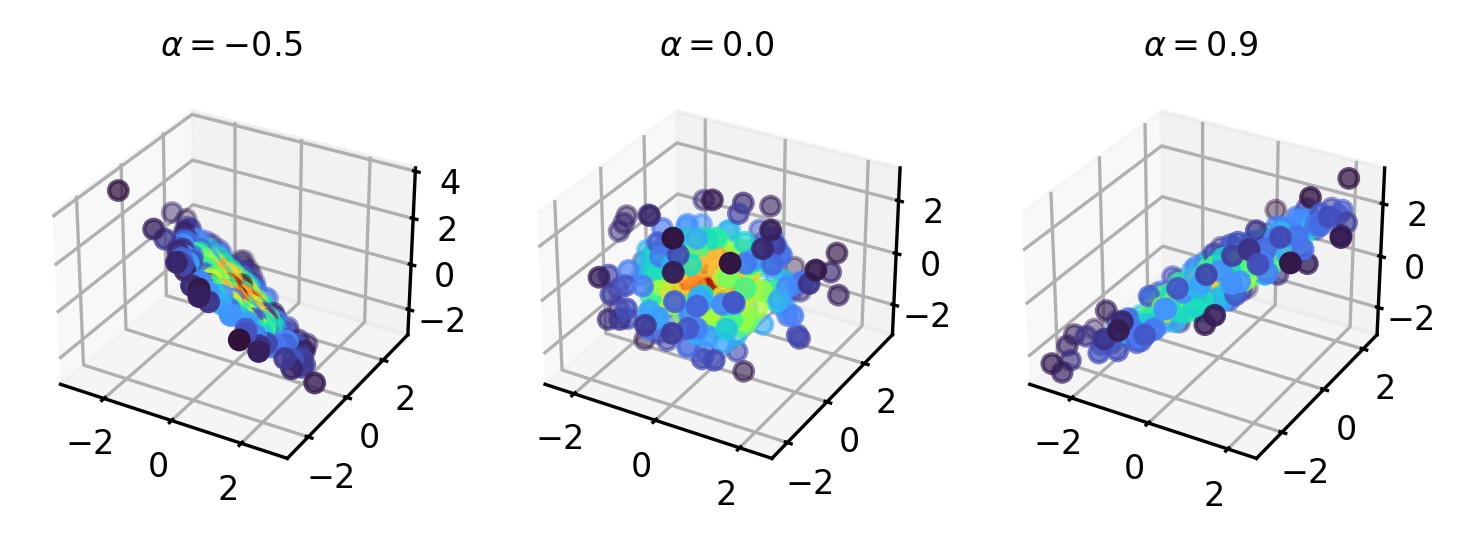
\includegraphics[width=15cm]{data_simulation/images/multivariate_normal/multivariate_normal.png}}
	\caption{Points drawn from a centered three-variate normal distribution with unit variance in the case of negative correlation (\emph{left}), zero correlation (\emph{center}) and positive correlation (\emph{right}). The points' color signify the probability density at that location.}
	\label{fig:data_simulation:multivariate_normal}
\end{figure}

For correlated noise, the problem at hand is similar: For multiple detectors, noise time-series $n_i$ should be simulated from a \emph{spectral matrix} $\underline{\underline{S_n}}$. This matrix contains each detector's noise PSD on its diagonal and the \emph{cross spectral densities} (CSDs) between detectors on the off-diagonal entries. For ET, that means three detectors, assuming the same PSD as in the uncorrelated case is each detector, $S_n^{ii} = S_n$ for $i=1,2,3$.
The CSDs are given by $S_n^{ij} = \alpha_{ij}\surd{S_n^{ii}S_n^{jj}} = \alpha_{ij} S_n$ with some correlation coefficient $\alpha_{ij}$. For the sake of simplicity, the same correlation is assumed between all detectors. Then, the spectral matrix can be written as
\begin{equation}
	\underline{\underline{S_n}} = \begin{pmatrix}
		S_n^{11} & S_n^{12} & S_n^{13} \\
		S_n^{21} & S_n^{22} & S_n^{23} \\
		S_n^{31} & S_n^{32} & S_n^{33}
	\end{pmatrix} 
	= \begin{pmatrix}
		1 & \alpha & \alpha \\
		\alpha & 1 & \alpha \\
		\alpha & \alpha & 1
	\end{pmatrix}\,S_n,
\end{equation}
with $\alpha$ bounded to a range between $-0.5$ and $1$. % One-liner, why that is the case
For a proof, see the \cite{PhysRevD.110.104060}.

An ansatz similar to Eq.~\ref{eq:data_simulation:uncorrelated_noise_dft_ansatz} is made for each detector's noise Fourier transform, 
\begin{equation}
	\tilde{n}_i(f) = a_i (x_i + iy_i).
\end{equation}
But now, the random variates $x_i$ and $y_i$ for each detector are not drawn independently of each other. Rather, vectors $\vec{x} = \begin{pmatrix} x_1 & x_2 & x_3 \end{pmatrix}^\intercal$ and $\vec{y} = \begin{pmatrix} y_1 & y_2 & y_3 \end{pmatrix}^\intercal$ are drawn from a \emph{multivariate} (in this case three-variate) normal distribution again with zero mean and unit variance, \emph{i.e.}, with a \emph{covariance matrix} that is given by
\begin{equation}
	\Sigma = \begin{pmatrix}
		1 & \alpha & \alpha \\
		\alpha & 1 & \alpha \\
		\alpha & \alpha & 1
	\end{pmatrix}.
\end{equation}
% \emph{i.e.}\ $x, y \sim \mathcal{N}(\mu=0, \Sigma)$
For a visualization of this distribution, see Fig.~\ref{fig:data_simulation:multivariate_normal}.
% Describe what we are seeing in this plot
Again, for each detector Eq.~\ref{eq:data_simulation:psd_relationship} should hold. Since $\langle x_i^2\rangle = 1$, the same formula for $a_i$ is recovered as in Eq.~\ref{eq:data_simulation:prefactor}. Then, the inverse Fourier transform yields the desired time-series.

In practice, a small positive correlation of $\alpha=0.1$ is assumed in the regime where seismic and Newtonian noise is dominant, which is below frequencies of \SI{10}{\hertz}. For higher frequencies $\alpha=0$, in which case the covariance matrix collapses to an identity matrix and the probability distribution effectively behaves as three independent normal distributions. A lower frequency cutoff of \SI{4}{\hertz} is applied, which means that the PSD is set to zero below that frequency. Furthermore, a sampling rate of \SI{2048}{\hertz} is chosen resulting in an upper resolution limit given by the Nyquist frequency, in this case \SI{1024}{\hertz}.  This is a reasonable resolution range, when considering BBH signals only. The inclusion of BNS signals in the simulation as well would necessitate a higher sampling rate. 
% The reasoning behind these frequency cuts has to do with the sort of signals that are simulated, which is the topic of the next chapter.
% TODO: plot noise with alpha=1 as sanity check, also plot realistic as is used in the simulations

\section{Gravitational Wave Signals}

It is important for the simulated dataset to cover all possible signal waveforms evenly such that when training neural networks no biases are learned. The shape of these waveforms will depend on a number of parameters, which are referred to as extrinsic and intrinsic. The former describe the signal source's location with respect to the detector reference frame and the latter are the intrinsic properties of the binary system, such as their masses.

\subsection*{Parameters}

\begin{figure}
	\centering
	\begin{minipage}{\textwidth}
		\centering
		\makebox[\textwidth]{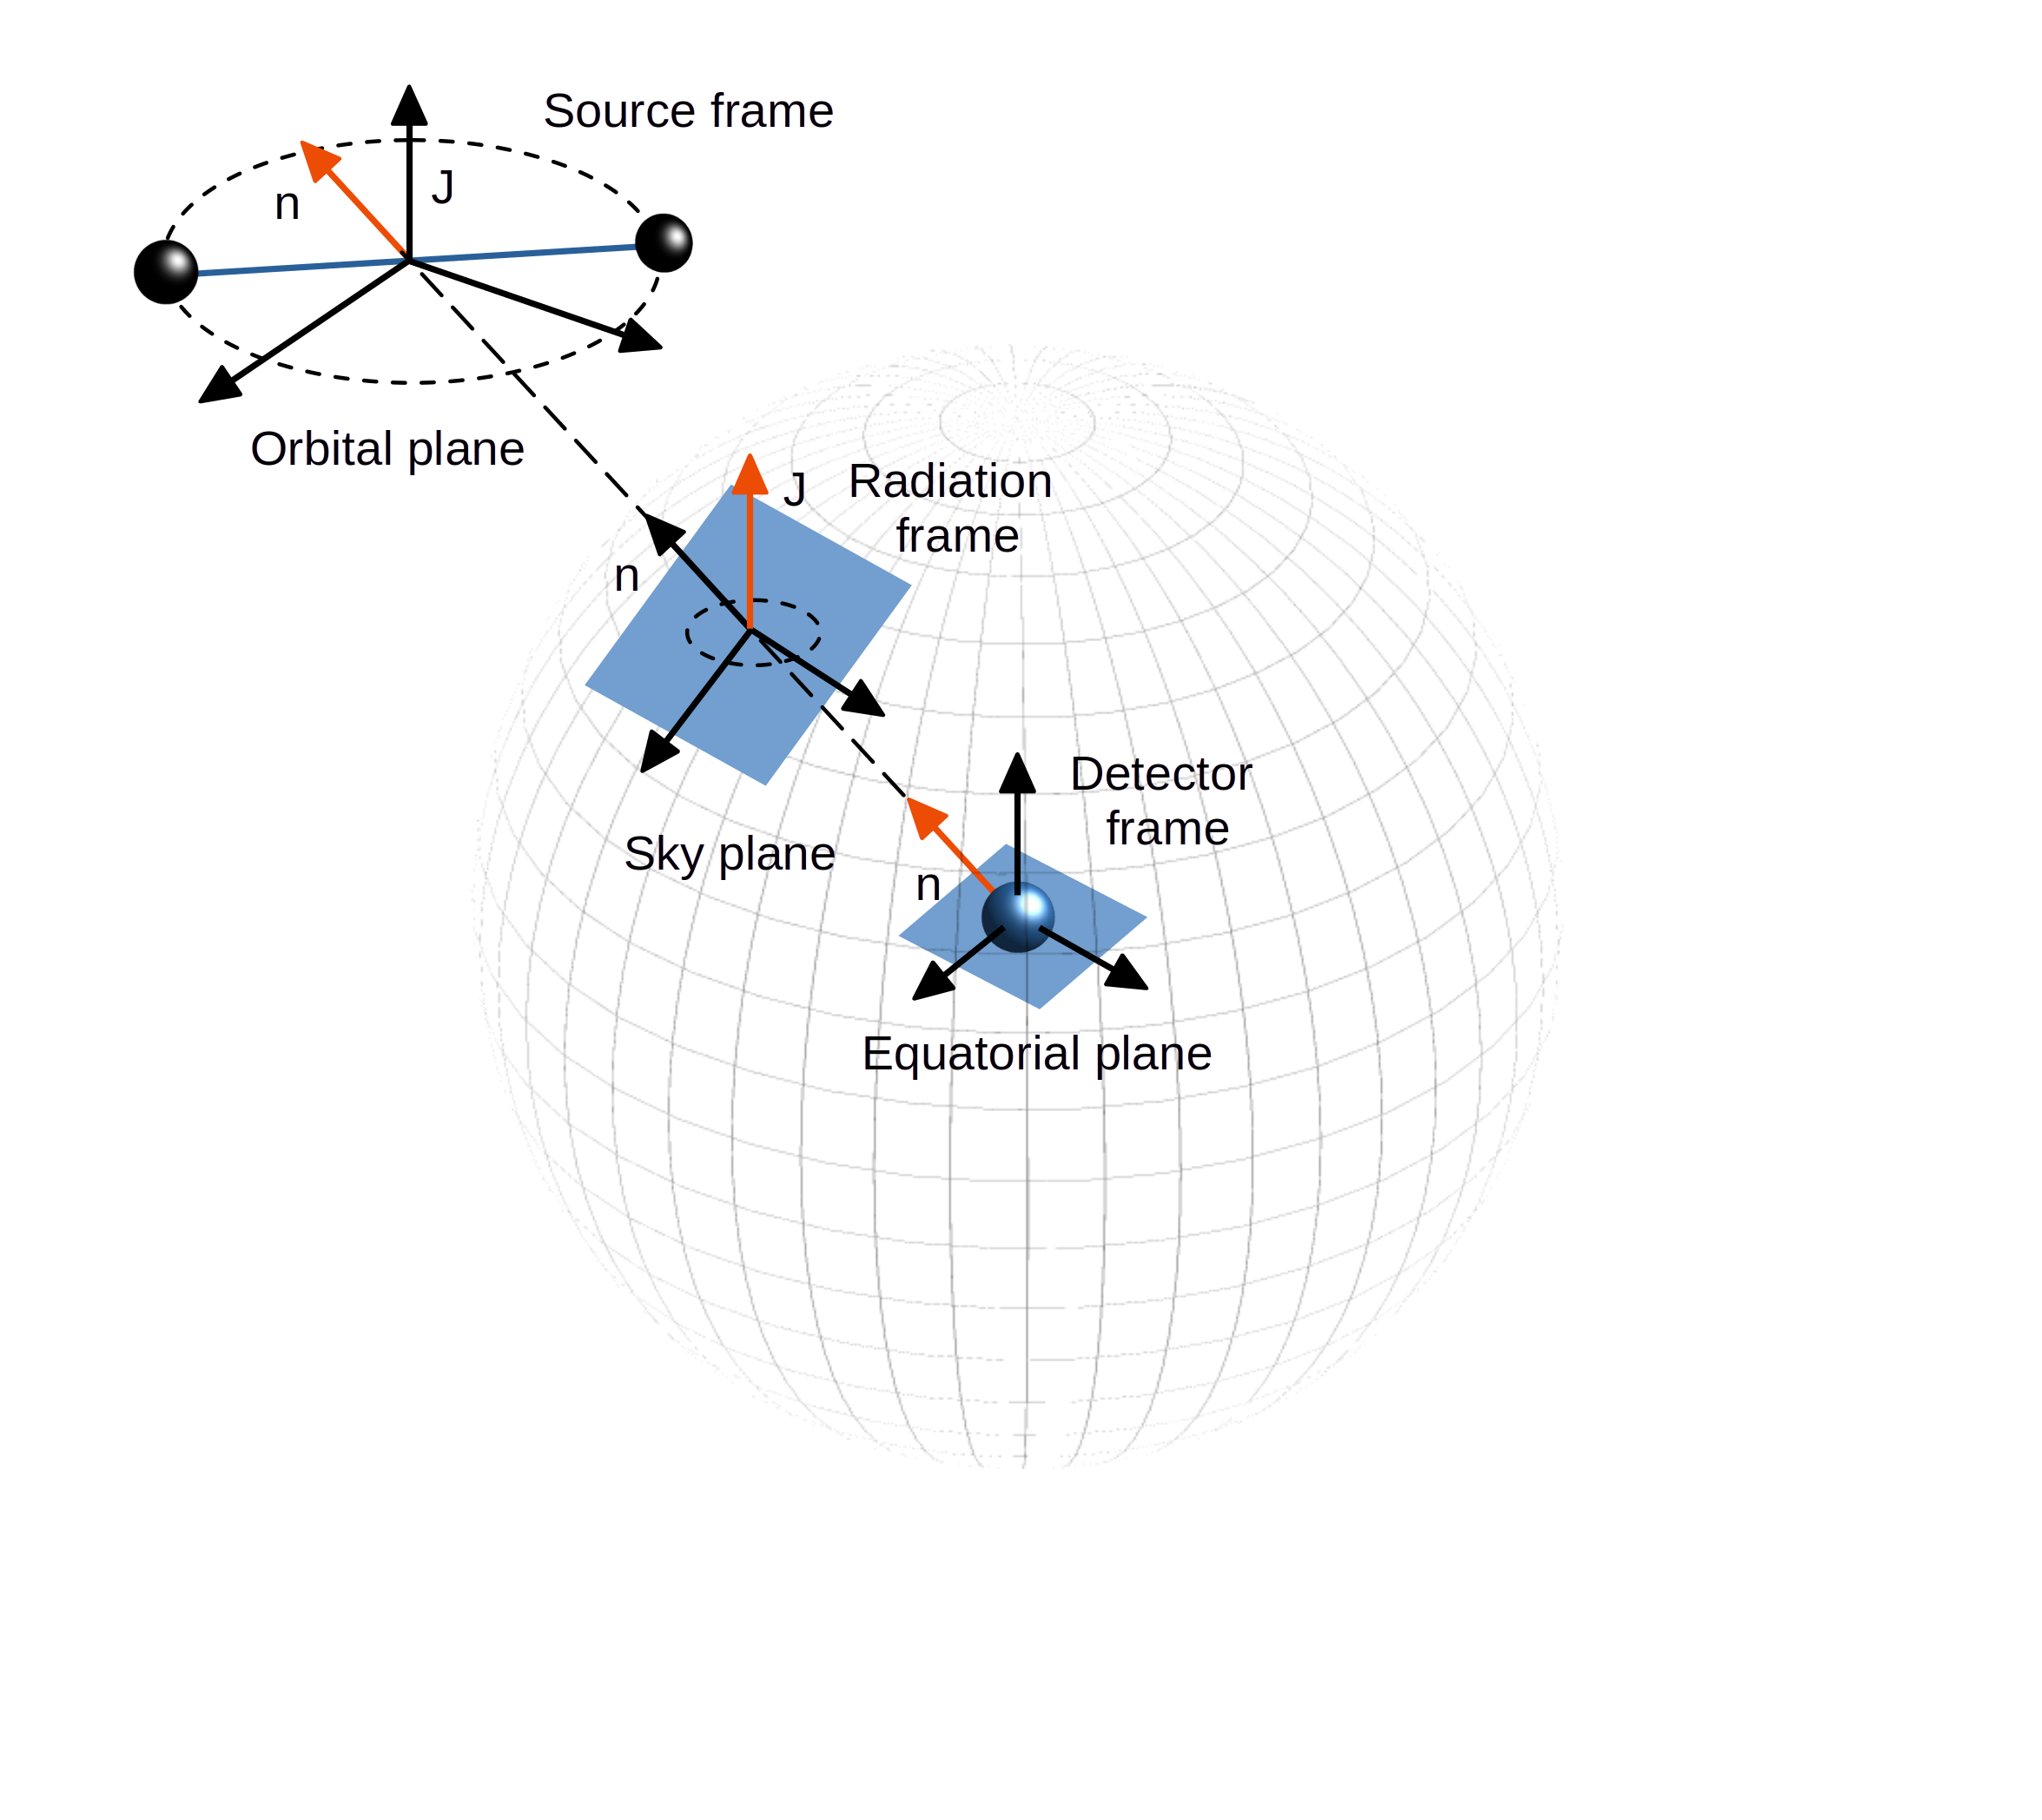
\includegraphics[width=10cm, trim=0 30cm 30cm 0, clip]{data_simulation/images/frames/frames_crop.png}}
		\caption{The three simulation frames. $\vec{n}$ is the line-of-sight vector that points towards the source. $\vec{J}$ denotes the binary's angular momentum vector.}
		\label{fig:data_simulation:frames}
	\end{minipage}
	\begin{minipage}{\textwidth}
		\centering
		\makebox[\textwidth]{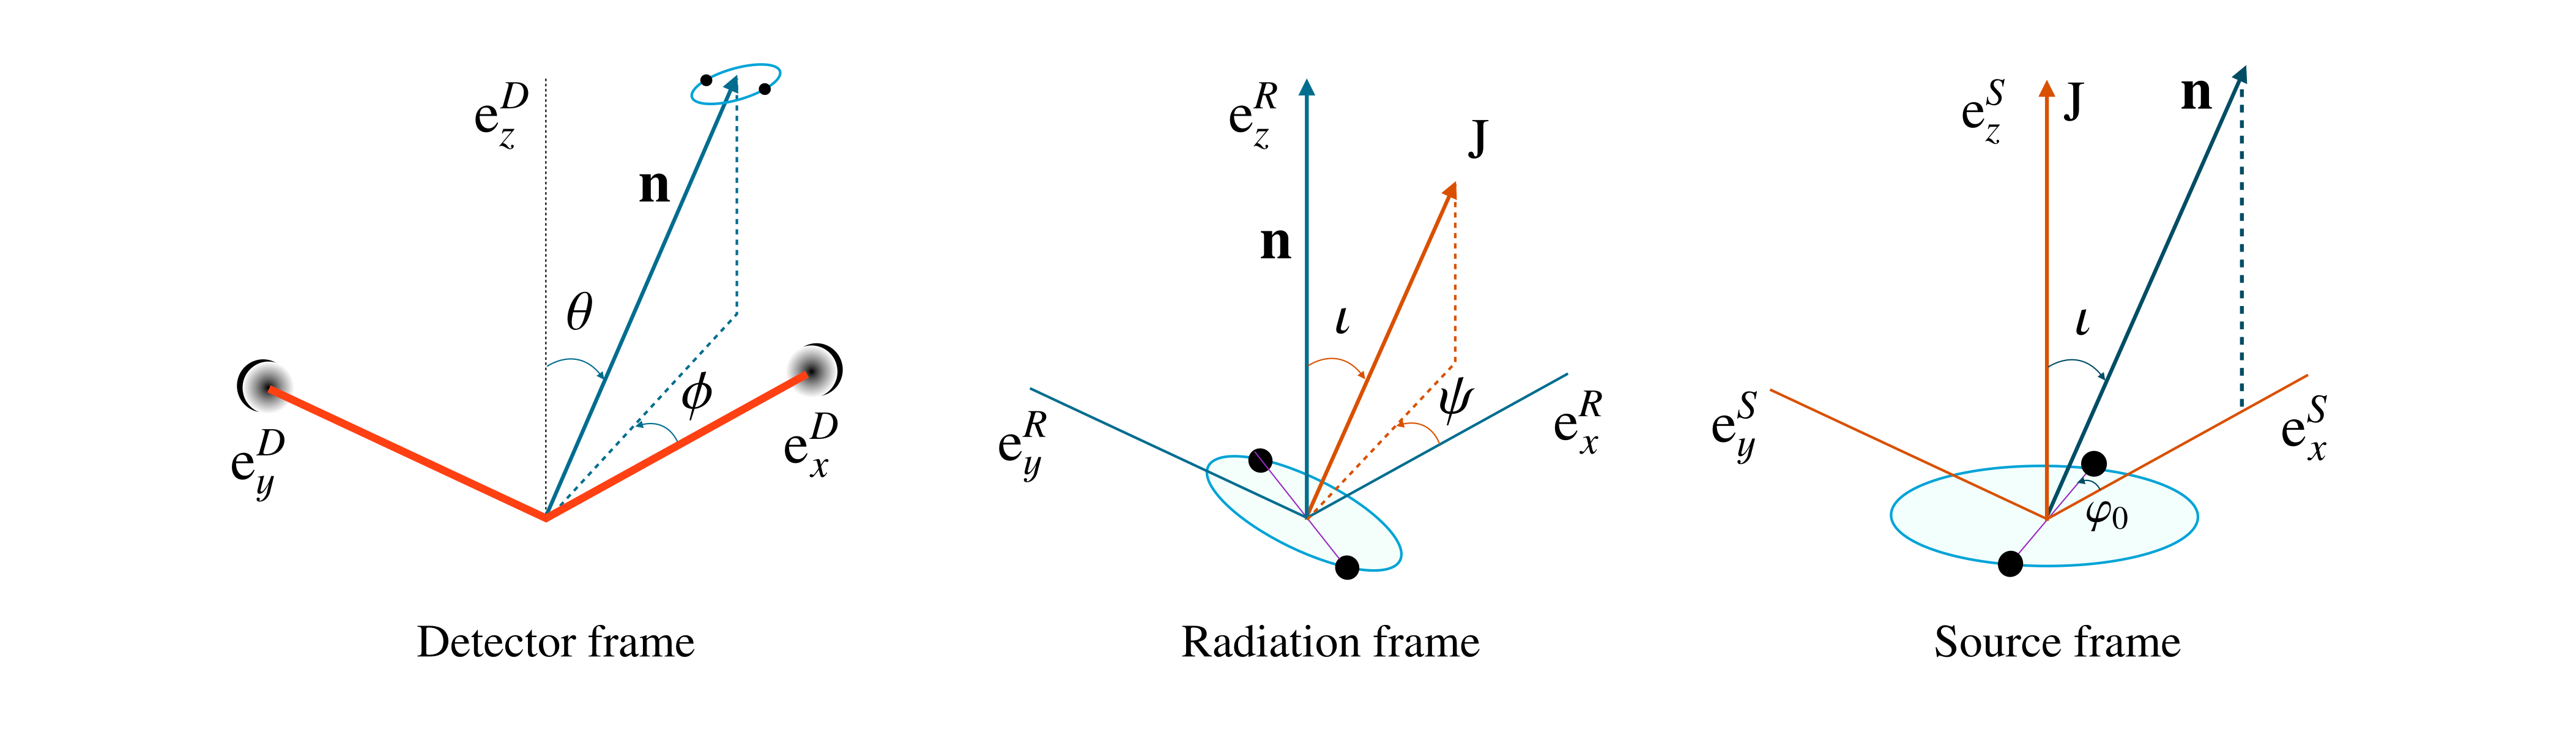
\includegraphics[width=18cm]{data_simulation/images/parameters/Detector-frame-The-two-orthogonal-arms-of-the-interferometer-form-the-x-and-y-axes-in_high_res.png}}
		\caption{The extrinsic parameters as defined within the three simulation frame. Here, the detector frame is defined by the interferometer geometry, which is not the convention this thesis follows. Taken from \cite{PhysRevD.90.124004}.}
		\label{fig:data_simulation:parameters}
	\end{minipage}
\end{figure}

The extrinsic parameters are defined through three simulation frames, the detector frame, the radiation frame and the source frame. In this thesis, the detector frame is the Equatorial coordinate system. This frame has a z-axis pointing towards the Earth's north pole, and an x-axis that points towards the March equinox. The y-axis is determined by the right circular convention.
The radiation frame can be thought of as the sky projection of the detector frame. Its z-axis is the line-of-sight vector towards the GW source. The x-axis is the projection of the detector frame's x-axis onto the sky plane, and the y-axis is again known by convention. The source frame has a z-axis pointing along the binary's orbital momentum vector. It x--y plane is the orbital plane, where the x-axis the projection of the line-of-sight vector.
See a schematic of the simulation frames in Fig.~\ref{fig:data_simulation:frames}.

There are a total of seven extrinsic parameters. The polar coordinates of the line-of-sight vector, \emph{i.e.}\ the inverse GW propagation direction, are the declination $\theta$ and the right ascension $\phi$. These two angles are defined with respect to the detector frame. 
The orientation of the binary with respect to the radiation frame yields two more parameters, the inclination $\iota$ and the polarization $\psi$. These are the polar angles of the source frame's z-axis, \emph{i.e.}\ the binary plane's normal vector, defined within the radiation frame. 
The other three parameters are the distance between detector and source $d$, as well as the coalescence time $t_\text{coa}$ and corresponding coalescence phase $\phi_\text{coa}$. The latter is the polar angle of primary mass in the source frame. The definition of the angle parameters are shown in Fig.~\ref{fig:data_simulation:parameters}.

The binary system has six intrinsic parameters. 
These include the two masses, the larger of which is called the primary mass $m_1$ by convention. (The other one is denoted $m_2$.) These masses can have non-zeros spins, which are described by the two vectors $\vec{S}_1$ and $\vec{S}_2$. The spins are defined within the source frame. In practice it is useful to define the dimensionless spin as $\vec{\chi}_i = \vec{S}_i / m_i^2$ with $|\vec{\chi}_i| < 1$ (in natural units that is).

\subsection*{Waveform Simulation}

For the simulation of gravitational wave signals from the inspiral, merger and ringdown of black hole binaries, the phenomenological model \emph{IMRPhenomD} \cite{PhysRevD.93.044007} is used as implemented by \emph{lalsimulation}. This is part of the LIGO Algorithm Library \cite{lalsuite}, which in turn is accessed via PyCBC.

These simulations take all the intrinsic parameters as inputs, which are the masses and spins.
The black hole mass distribution is modeled after CBC detections made by the second-generation network so far (see Fig.~\ref{fig:einstein_telescope:population}). Both black hole masses sampled uniformly in $[\SI{10}{\solarmass}, \SI{80}{\solarmass}]$, where the larger is the primary mass $m_1$ and the other $m_2$. 
This roughly corresponds to coalescence frequencies in a range of $[\SI{30}{\hertz}, \SI{220}{\hertz}]$ (see Eq.~\ref{eq:theory_of_gravitational_waves:max_freq_approx}), making the chosen sampling rate of \SI{2048}{\hertz} appropriate.
In the scope of this work, only aligned spin BBHs are considered, which means $\chi^i_x = \chi^i_y = 0$ and $\chi^i_z \geq 0$. The z-component of the spin is sampled uniformly in $[0, 0.998]$ with an upper limit that equals the Thorne limit. 

\begin{figure}
	\centering
	\begin{minipage}{\textwidth}
		\centering
		\makebox[\textwidth]{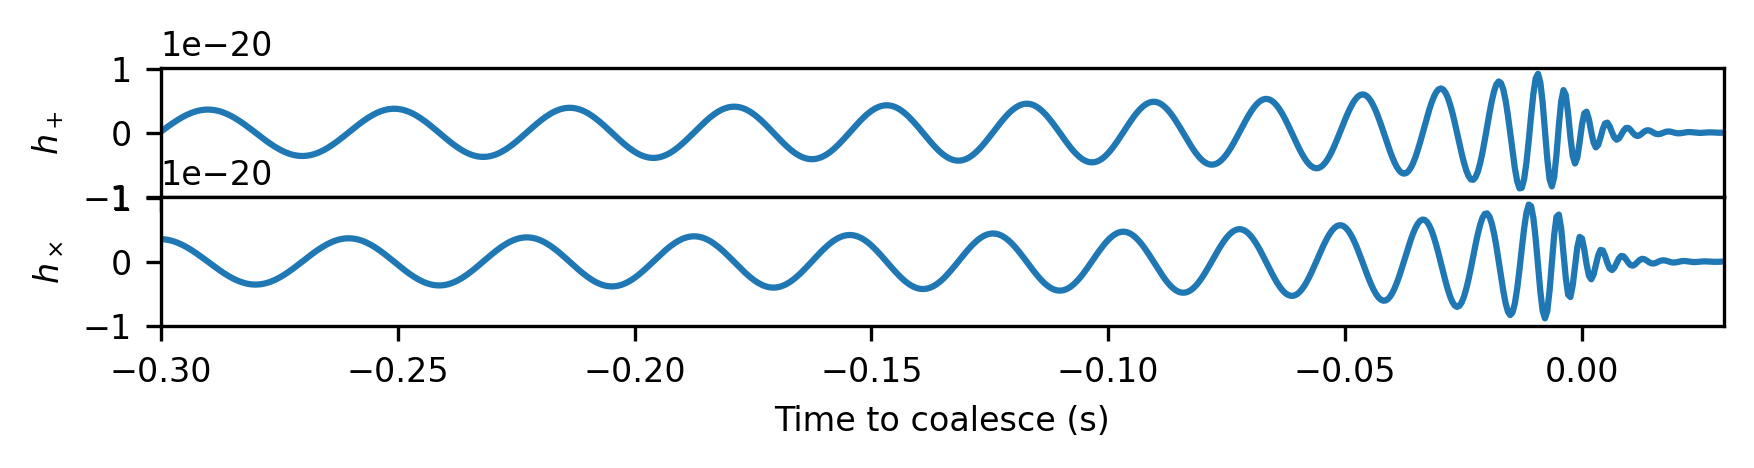
\includegraphics[width=15cm]{data_simulation/images/waveforms/waveform.png}}
		\caption{The plus and cross polarization strain of a GW signal emitted by a black-hole binary with masses $m_1 = \SI{50}{\solarmass}$, $m_2 = \SI{40}{\solarmass}$ and spins $\chi^1_z = 0.73$, $\chi^2_z = 0.43$ at a distance of \SI{100}{\mega\parsec}.}
		\label{fig:data_simulation:waveform}
	\end{minipage}
	\begin{minipage}{\textwidth}
		\centering
		\makebox[\textwidth]{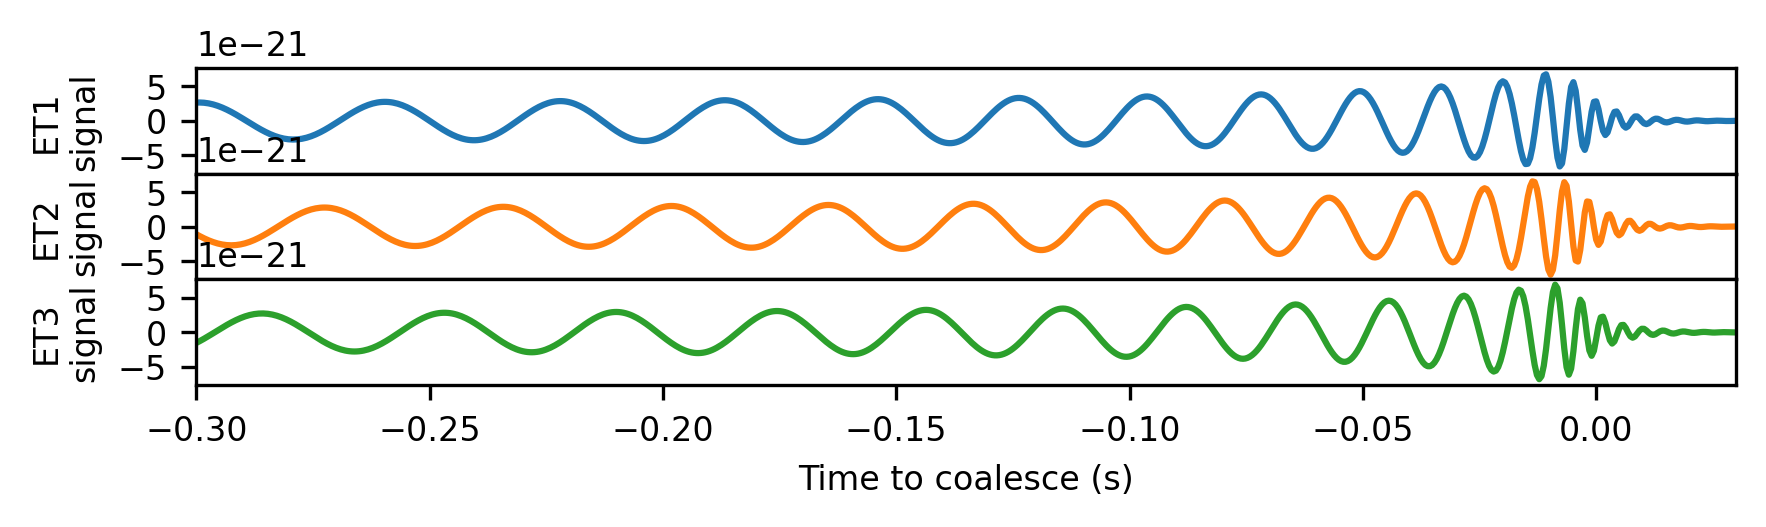
\includegraphics[width=15cm]{data_simulation/images/waveforms/projection.png}}
		\caption{The same GW signal from Fig.~\ref{fig:data_simulation:waveform} projected onto the three ET detectors as having a sky location $\phi = \SI{263}{\degree}$, $\theta = \SI{56}{\degree}$ and a polarization that is $\psi = \SI{78}{\degree}$.}
		\label{fig:data_simulation:projection}
	\end{minipage}
\end{figure}

The radiation pattern of the binary also depends on the binary's inclination and the coalescence phase. The inclination $\iota$ is sampled from a sine distribution with a probability density function proportional to $\sin{x}$ for $x$ in $[0, \pi]$.
The coalescence phase $\varphi_\text{coa}$ is sampled uniformly in $[0, 2\pi)$. 
Another simulation input parameter is the source distance. Since only the total strain amplitude depends on that distance and since there will be a rescaling step later anyway, the exact value is arbitrarily set to \SI{100}{\mega\parsec}. 
The simulation employs a lower frequency cutoff, which is the starting frequency of the waveform, which is set to \SI{4}{\hertz}. 
A waveform with all these parameters sampled accordingly can be seen plotted in Fig.~\ref{fig:data_simulation:waveform}.

\subsection*{Antenna Projection}

% for some reasons lalsimulation implements ET as being at 43.6314°N 10.5045°E, which is the site of VIRGO, see Einstein Telescope pre-site selection detector locations technical document LIGO DCC: T1400308

The simulated waveform are projected onto the ET interferometers to yield the GW strain according to Eq.~\ref{eq:einstein_telescope:antenna_functions}.
A PyCBC routine is relied upon to handle these antenna projections. The package implements ET according to \cite{T1400308} as three detectors in a triangular configuration with \SI{10}{\kilo\meter}-long arms. The detector is located at \SI{43.6314}{\degreeLat} \SI{10.5045}{\degreeLong}, which is the site of Virgo. 

PyCBC takes as input the detector GPS location, the GW signal sky position (in the equatorial frame) and the polarization.
In the simulation, the sky location is sampled uniformly. This means, the declination $\theta$ is sampled from a sine distribution and the right ascension $\phi$ uniformly in $[0, 2\pi)$. The GW polarization $\psi$ is sampled in $[0, 2\pi)$.
The routine further depends on the GW arrival time, for which PyCBC calculates the revolution of the Earth and updates the detector GPS location accordingly.
Since the GW sky position is sampled uniformly anyway, the arrival time is arbitrarily chosen to be zero. 
A GW signal that is projected as such is plotted in Fig.~\ref{fig:data_simulation:projection}.

\subsection*{Waveform Tapering}

The waveform simulation starts at the lower frequency cutoff, which is set to \SI{4}{\hertz}. This results in an \enquote{abrupt} jump in strain amplitude once the signal sets in which is an unphysical signature a neural network might pick up on easily. To mitigate this a tapering of the waveform is implemented by multiplying with a one-sided Tukey window:
\begin{equation}
	w(x) = \begin{cases}
		\frac{1}{2}(1-\cos{\frac{2\pi}{\alpha}\,x}) & \text{if } 0\leq x <\frac{\alpha}{2}\\
		1 & \text{if } \frac{\alpha}{2}\leq x<1.
	\end{cases}
\end{equation}
Here, $x$ is in units of total waveform length, \emph{i.e.}, $x=0$ corresponds to the beginning and $x=1$ to the end of the waveform. $\alpha = 1/4$ is chosen which means that the smoothing extends up to one eighth of the waveform. This trick is borrowed from \cite{PhysRevD.100.063015}.

\subsection*{SNR Rescaling}

In order to ease training for the neural networks, the dataset should include signals with a \enquote{loudness} that is evenly distributed. Preferably in a range, where detection is neither impossible nor trivial. To achieve this, the waveforms are rescaled by some factor $\beta$. 
A measure for the signal loudness is the optimal SNR (see Sec.~\ref{sec:matched_filtering}). This is denoted $\rho$ instead of $\rho_\text{opt}$ from now on. For multiple detectors the optimal SNR is,
\begin{equation}
	\rho^2 = \rho^2_1 + \rho^2_2 + \rho^2_3,
\end{equation}
with $\rho^2_i$ denoting the SNR of each of the three ET detectors. The individual detector SNR is given by Eq.~\ref{eq:matched_filtering:snr}, or in discrete form by,
\begin{equation}
	\rho^2_i = 4 \sum_j \Delta f \frac{|\tilde{h}_i(f_j)|^2}{S_n(f_j)}.
\end{equation}
Rescaling the signal amplitude by some positive factor $h_i(t)\rightarrow\beta h_i(t)$, means that the Fourier transform scales as, $\tilde{h}_i(f)\rightarrow\beta\tilde{h}_i(f)$. Thus, the individual detector SNRs scale as, $\rho_i\rightarrow\beta\rho_i$ and finally the total SNR as, $\rho\rightarrow\beta\rho$. That is to say, the signal waveform can just be rescaled by some positive prefactor to ensure a desired SNR. This prefactor is then given by $\beta = \rho / \rho'$, where $\rho$ is the desired SNR and $\rho'$ the SNR prior to rescaling. This desired SNR is sampled uniformly in $[5, 15]$. Signals with an SNR of $\sim5$ are more or less not detectable with matched filtering. For SNRs over $\sim10$, matched filtering reaches close to perfect detection ratios \cite{Nitz_2017}. GW150914 was observed with an total SNR of $24$ \cite{PhysRevLett.116.061102}.

In the case of correlated noise, this SNR formula does not hold anymore. Instead, as proposed in \cite{PhysRevD.110.104060}, the SNR is given by,
\begin{equation}
	\label{eq:data_simulation:correlated_snr}
	\rho^2 = 4 \Delta f \sum_k \sum_{i,j}
	\tilde{h}_i(f_k)^*(\underline{\underline{S_n}}^{-1})_{ij}(f_k)\tilde{h}_j(f_k),
\end{equation}
where $i,j$ sum over all detector combinations and $\underline{\underline{S_n}}^{-1}$ is the inverse spectral matrix,
\begin{equation}
	\underline{\underline{S_n}}^{-1} = \frac{1}{2\alpha^2 - \alpha - 1}
	\begin{pmatrix}
		-\alpha-1 & \alpha & \alpha \\
		\alpha & -\alpha-1 & \alpha \\
		\alpha & \alpha & -\alpha-1
	\end{pmatrix} \frac{1}{S_n}.
\end{equation}
Fortunately, since $\rho^2 $ is just a linear combination over all $\tilde{h}_i(f)^*\tilde{h}_j(f)$, rescaling with $\beta = \rho / \rho'$ is still valid. The difference is only that the pre-rescaling SNR $\rho'$ is calculated using the adapted SNR formula, \emph{i.e.}\ Eq.~\ref{eq:data_simulation:correlated_snr}.

\section{Samples and Datasets}

The datasets are built from multiple samples. Each sample resembles ET detector stream data of some length. To this end, partially correlated noise of that length is simulated and a number of GW signals are \emph{injected}, which simply means added. The waveform parameters are drawn randomly as described previously. For better clarity, the parameter distributions are restated in Tab.~\ref{tab:data_simulation:waveform_parameters}. The signals are injected with random coalescence times, covering the whole length of the detector stream. 

\begin{table}[]
	\centering
	\caption{Simulation waveform parameter distributions.}
	\label{tab:data_simulation:waveform_parameters}
	\begin{tabular}{l c l}
		\toprule
		\multicolumn{2}{c}{Waveform parameter} & Distribution \\
		\midrule
		Masses & $m_1$, $m_2$ 
		& $\text{Uniform}(\SI{10}{\solarmass}, \SI{80}{\solarmass})$ \\
		Non-aligned spins & $\chi_x$, $\chi_y$
		& $0$ \\
		Aligned spins & $\chi_z$
		& $\text{Uniform}(0, 0.998)$ \\
		Sky position & $\theta$, $\phi$
		& $\text{Sine}(0, \pi)$, $\text{Uniform}(0, 2\pi)$ \\
		Inclination and polarization & $\iota$, $\psi$
		& $\text{Sine}(0, \pi)$, $\text{Uniform}(0, 2\pi)$ \\
		Coalescence phase & $\varphi_\text{coa}$
		& $\text{Uniform}(0, 2\pi)$ \\
		Optimal SNR & $\rho$
		& $\text{Uniform}(5, 15)$ \\
		
		\bottomrule
	\end{tabular}
\end{table}
In this work, the task of detecting multiple long-duration signals will be split in two steps. First, the simplified problem of detecting one long-duration signal per sample is considered. This allows testing different architectures, while increasing the sample length. To fit a full BBH waveform, a final sample length of $\approx\SI{1}{\minute}$ is aimed for. Multiple datasets with increasing length are constructed. For better comparability, training datasets will always consist of \SI{1}{\mega\nothing} samples in this thesis. Since there is only up to one signal per sample, this task can be simplified to a \emph{binary-classification} problem. In this case, the network will predict one number per sample that signifies whether there is signal in the given detector stream or not. Samples with no injection will be labeled \emph{negative}, \emph{i.e.}\ $0$, and samples with an injected signal \emph{positive}, \emph{i.e.}\ $1$. To avoid learned biases, the dataset will be constructed evenly, that is, half of the samples will be positive and the other half negative.

\begin{figure}
	\centering
	\makebox[\textwidth]{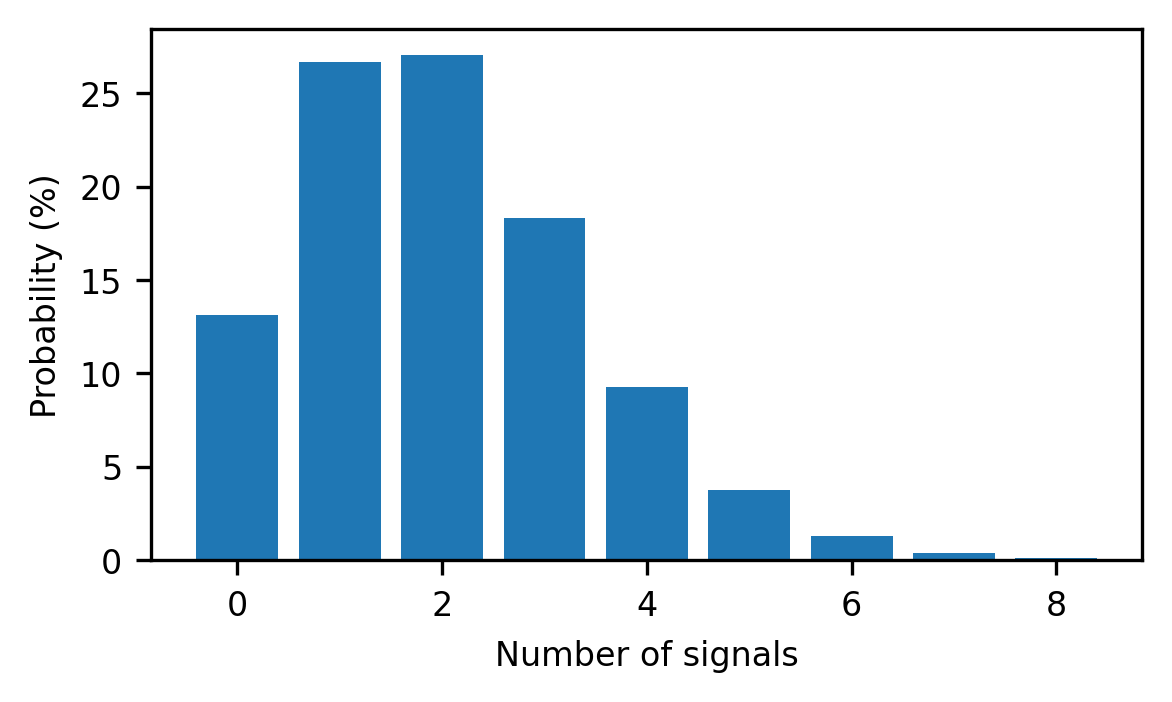
\includegraphics[width=10cm]{data_simulation/images/poisson/poisson}}
	\caption{Probability of $n$ number of signals in a \SI{64}{\second} sample of ET detector stream, assuming the higher event rate estimate of \SI{E+6}{\per\year}.}
	\label{fig:data_simulation:poisson}
\end{figure}

\begin{figure}
	\centering
	\makebox[\textwidth]{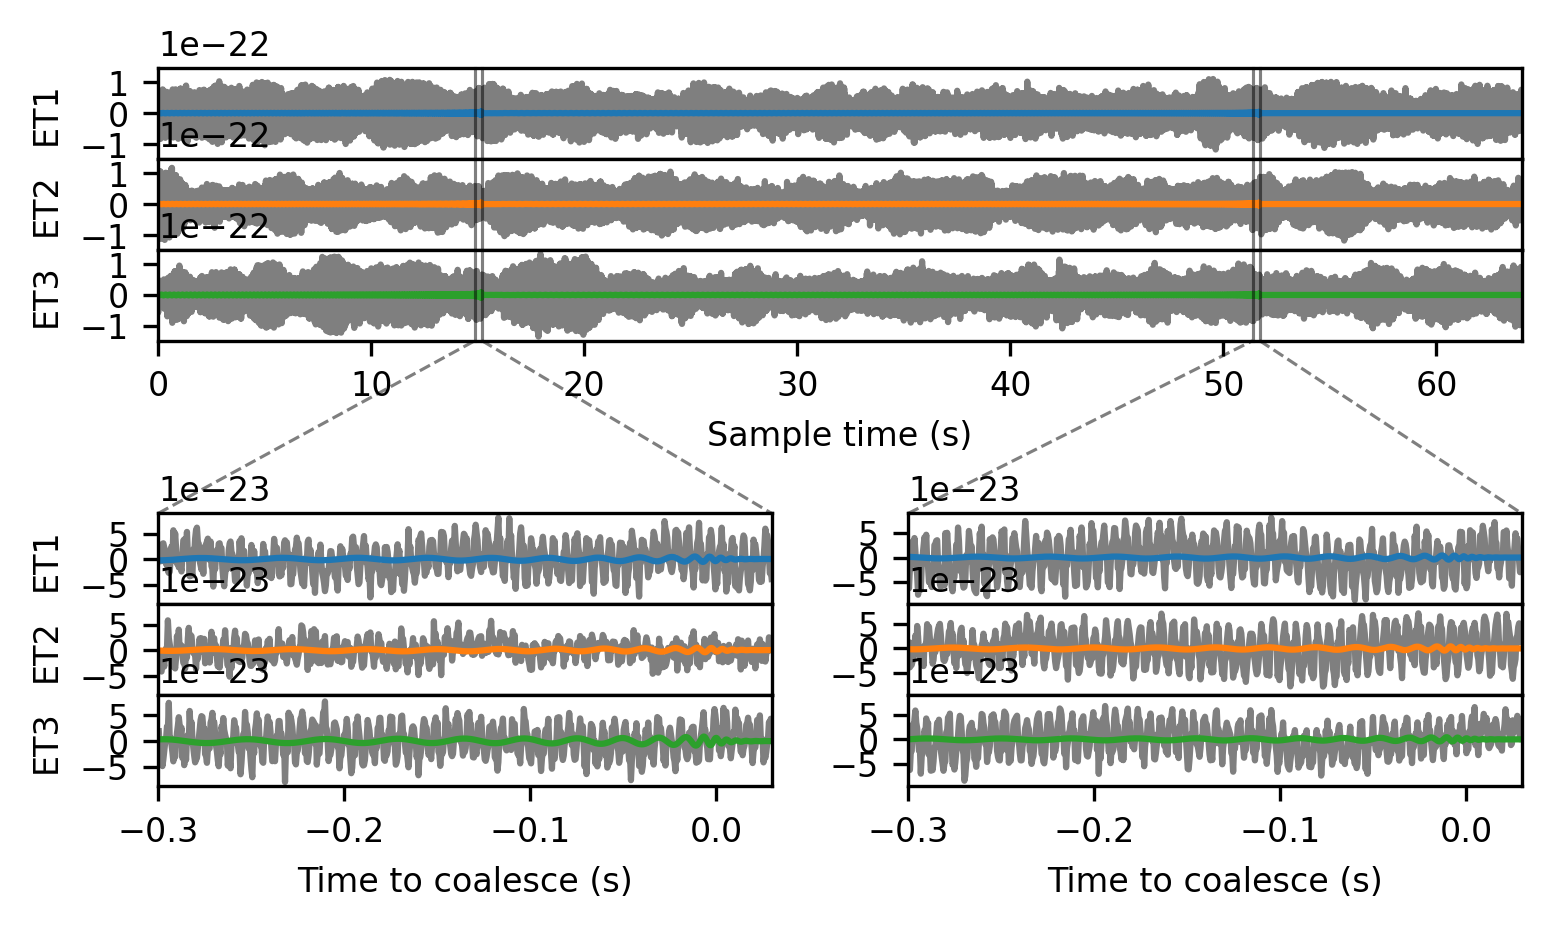
\includegraphics[width=15cm]{data_simulation/images/waveforms/injection.png}}
	\caption{Sample with two injected signals. The total strain is plotted in gray, and the signal contribution in color. The first signal has an SNR of $\approx6.4$, and the second one has $\approx9.1$.}
	\label{fig:data_simulation:injection}
\end{figure}

\begin{figure}
	\centering
	\makebox[\textwidth]{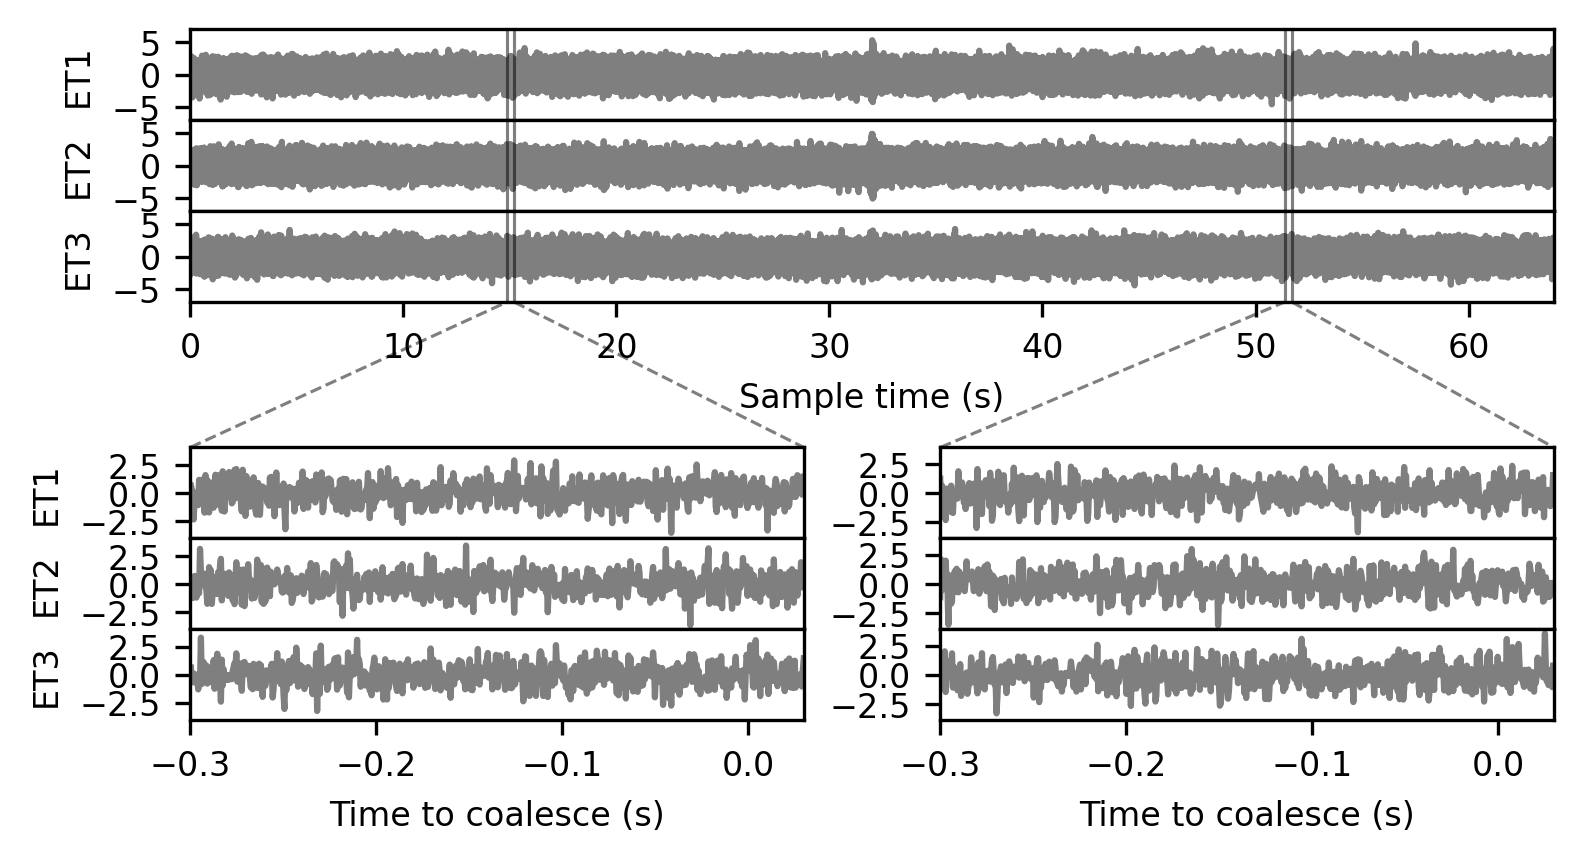
\includegraphics[width=15cm]{data_simulation/images/waveforms/sample.png}}
	\caption{The same sample as in Fig.~\ref{fig:data_simulation:injection} after whitening, band-passing and standardizing. This resembles the data that neural networks are trained on in this work.}
	\label{fig:data_simulation:sample}
\end{figure}

The second step deals with multiple such long-duration waveforms in a $\SI{64}{\second}$ sample. This case is treated similar to an \emph{object detection} task, where the network should predict multiple signals along with their coalescence time. To cover all cases evenly and ensure no biases are learned, the number signals per sample is sampled \emph{uniformly} in $[0, 6]$. The maximum of six signals is justified by the expected event rate in ET, which is up to $\lambda=\SI{E+6}{\per\year}$ signals. This is a Poissonian process, thus the probability of $n$ signals in one sample of length $T$ is,
\begin{equation}
 	P(n) = \frac{(\lambda\,T)^n}{n!}\,\e^{-\lambda\,T}.
\end{equation}
The distribution is visualized in Fig.~\ref{fig:data_simulation:poisson}. By choosing a maximum of six signals, most relevant cases are covered. See an example sample with two injected signals in Fig.~\ref{fig:data_simulation:injection}. Note that this neglects the simulation of signals with a merger time outside the sample window.

\section{Post-Processing}

Three post-processing steps are performed on the samples.
First, the data is \emph{whitened}. This step aims to turn the colored noise power spectrum into a white one, which is constant over the whole frequency regime. In theory, this can be achieved by down-weighting the strain's Fourier coefficients $\tilde{s}(f)$ by the noise amplitude spectral density, \emph{i.e.}\ the square root power spectral density $S_n$: 
\begin{equation}
	\tilde{s}'(f) = \frac{\tilde{s}(f)}{\sqrt{S_n(f)}}, 
\end{equation}
such that $S_n'(f) = 2\Delta f|\tilde{s}'(f)|^2 = 1$ in the absence of a signal.

In GW searches, the exact noise PSD is not known \emph{a priori} of course, and has to be estimated from the detector stream instead. To this end, an adaption from Welch's method is used, as implemented in PyCBC \cite{alex_nitz_2023_10013996}. This method splits the given detector strain into $N$ overlapping segments of some duration and with a stride that is half that duration. For each segment $i$, the PSD is computed as,
\begin{equation}
	S_n^i(f) = 2\Delta f|\tilde{s}^i(f)|^2.
\end{equation}
Then, an estimate of the noise PSD is the \emph{median} over all segments,
 \begin{equation}
 	S_n(f) = \frac{1}{\alpha}\,\text{median}(S_n^1(f), S_n^2(f), \dots), 
 \end{equation}
with a correction factor $\alpha = \sum_{i=1}^N (-1)^{i+1}/i$. The median instead of the mean is used to ensure that only the \emph{noise} PSD is estimated. The latter might be biased towards larger values in the presence of gravitational wave signals. 

In this thesis, the PSD is estimated for each detector and each sample separately.
This roughly mimics the procedure in real searches, where the PSD estimate is adjusted constantly.
Since the samples of some of the datasets are only a few seconds short, they are always simulated with some minimum length, over which the PSD is estimated, and later cut to the desired sample length. The minimum length is at least \SI{16}{\second} or twice the desired sample length. The extra is padded to both ends of the sample symmetrically, since the whitening procedure introduces corruption at both edges.

As another post-processing step the data is band-passed. The waveform fade-on can introduce frequency contributions below the frequency cut-off of \SI{4}{\hertz}, which might be a giveaway for the presence of a GW signal in the sample. Thus, the data is high-passed above \SI{4}{\hertz}. As this step also causes corruption at both ends of the sample, similar to whitening, the band-passing will be applied before cutting to the desired sample length.

The final processing step is standardizing the data. This is a common and often necessary data preparation step in a machine learning context, which ensures inputs with zero mean and unit variance. This is done for multiple samples at once, and for each detector  $i$ separately,
\begin{equation}
	s'_i(t) = \frac{s_i(t)-\mu_i}{\sigma_i},
\end{equation}
where $\mu_i$ and $\sigma_i$ denote the mean and standard deviation. These are computed over \SI{4096}{\nothing} samples each. See a post-processed sample in Fig.~\ref{fig:data_simulation:sample}. 
% The data includes whitening artefacts in the middle of each sample. These are caused by the harmonics of the noise PSD.

